\section {Photo-thermal time}
Photo-thermal time is a simple extension of the day-degree concept. You just weigh the  number of day-degrees accrued in a day by the length of the day (from sunrise to sunset). Since photo-thermal time is not included in the standard \US, we will use it as an example of how to implement you own box classes in \US.

\subsection {Getting started}
To get started with \CPP-coding, you first need to complete the following steps:
\begin{enumerate}
\item Download and install Qt Creator (\iref{ch:install-qt})
\item Download and unpack the Boost libraries (\iref{ch:install-boost})
\item Download and unpack the latest \US\ source code (\iref{ch:workflow})
\item Build \US\ from source code (\iref{ch:workflow})
\end{enumerate}

\subsection {Copying an existing class}
For your first box class, we will use the code of an existing class as a starting point. In fact, even later on, most modellers will find this the easiest approach.

Before you create a new box class, you must decide to which plug-in it should belong. The \US\ source code comes with the \concept{student plug-in} which is provided as a starting point for your own plug-in development. You can always, later on, rename the student plug-in to reflect the specific topic of your plug-in (\todo{to be explained}).

You can find the source code for the student plug-in in the \devhomeexplained{src/plugins/student} folder. It comes with the source code for two classes \code{Fibonacci} and \filename{Jump} (\iref{qt-creator-student-files-1})

\begin {figure} [ht]
\centering
\tikzstyle{every node}=[draw=black,anchor=west]
\begin{tikzpicture}[%
  grow via three points={one child at (0.5,-0.7) and
  two children at (0.5,-0.7) and (0.5,-1.4)},
  edge from parent path={(\tikzparentnode.south) |- (\tikzchildnode.west)}]
  \node {student}
   child {node {fibonacci.cpp}}
   child {node {fibonacci.h}}
   child {node {jump.cpp}}
   child {node {jump.h}}
   child {node {student.pro}}
 ;
\end{tikzpicture}
\caption{Files in the \filename{student} project of the \US\ source code.}
\label{qt-creator-student-files-1}
\end{figure}

Following common \CPP\ practice, the source code for each class is split into two files: the header file (\filename{.h}) and the source file (\filename{.cpp}). The fifth file is the \concept{project file}. It contains a list of the files included in the project and further details about which software product should be built from the project, in this case, a plug-in library. 

Let's call your new class \code{DayLengthScale}. To prepare for that, copy the files \filename{fibonacci.h} and \filename{fibonacci.cpp} into the corresponding files  
\filename{\hbox{day_length_scale.h}} and \filename{\hbox{day_length_scale.cpp}}. Why I put underscores in the file names? It is just an old habit. Feel free to follow your own ideas about name-giving.

\begin {figure} [ht]
\centering
\tikzstyle{every node}=[draw=black,anchor=west]
\begin{tikzpicture}[%
  grow via three points={one child at (0.5,-0.7) and
  two children at (0.5,-0.7) and (0.5,-1.4)},
  edge from parent path={(\tikzparentnode.south) |- (\tikzchildnode.west)}]
  \node {student}
   child {node {day_length_scale.cpp}}
   child {node {day_length_scale.h}}
   child {node {fibonacci.cpp}}
   child {node {fibonacci.h}}
   child {node {jump.cpp}}
   child {node {jump.h}}
   child {node {student.pro}}
 ;
\end{tikzpicture}
\caption{Files in the student project with two new files added for the \code{DayLengthScale} class.}
\label{qt-creator-student-files-2}
\end{figure}

\subsection {Code your class in Qt Creator}
In Qt Creator open the \filename{UniSim2.pro} project file. You will find it in the \devhome\ folder. First time you open this project, Qt Creator will take a while to digest it. Keep an eye on the lower right corner and wait until you see a full green bar.
The left-hand panel has now been populated with an outline of the complete \US\ source code (\iref{fig:qt-creator-projects}). The precise contents may vary due to developments later than this screen shot.

\begin{figure}
\centering
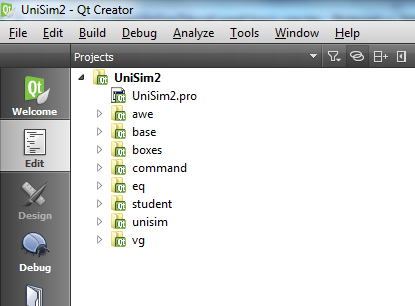
\includegraphics[scale=0.7]{graphics/qt-creator-projects}
\caption{Projects panel for \filename{UniSim2.pro} outlining the complete \US\ source code.}
\label{fig:qt-creator-projects}
\end{figure}

Click the \gui{student} entry to unfold it and under that, unfold the \gui{Headers} and \gui{Sources} entries too (\iref{fig:qt-creator-projects-student-1}). You will notice that the header and source files are represented, except that the \code{DayLengthScale} header and source files are not there yet. It is because we need to add them to the \filename{student} project file to make them part of the project.

\begin{figure}
\centering
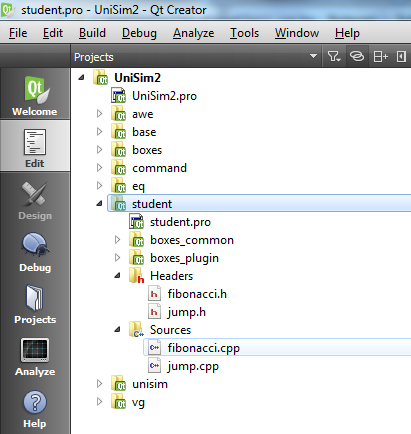
\includegraphics[scale=0.7]{graphics/qt-creator-projects-student-1}
\caption{Projects panel with parts of the student project unfolded.}
\label{fig:qt-creator-projects-student-1}
\end{figure}

To edit the \filename{student} project file double-click the \gui{student.pro} entry in the left-hand panel (\iref{fig:qt-creator-projects-student-1}). In the editor window you will see the contents of the \filename{student.pro} file. For now, we will focus on the \code{HEADERS} and \code{SOURCES} list that you find at the end of the file (\iref{fig:qt-creator-project-file-1}).

\begin{figure}
\centering
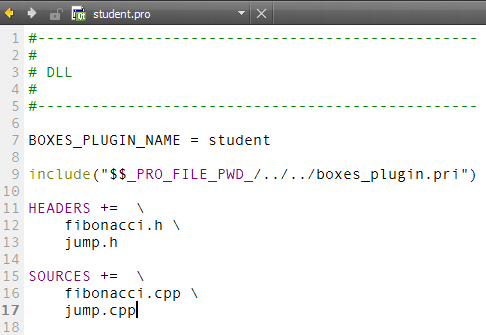
\includegraphics[scale=0.7]{graphics/qt-creator-project-file-1}
\caption{The initial contents of the student project file (\filename{student.pro}) in the \US\ source code.}
\label{fig:qt-creator-project-file-1}
\end{figure}

First, note that in these two lists, all lines except for the last one, end with a backslash. The backslash means 'list continued on next line' so do keep the backslashes like that, whenever you edit the list. Type in the file names of the \filename{day_length_scale} header (\filename{.h}) and source (\filename{.cpp}) file (\iref{fig:qt-creator-project-file-2}). Save the file and note that in the left-hand panel, new \gui{day_length_scale.h} and \gui{day_length_scale.cpp} entries appear (\iref{fig:qt-creator-projects-student-2}).

\begin{figure}
\centering
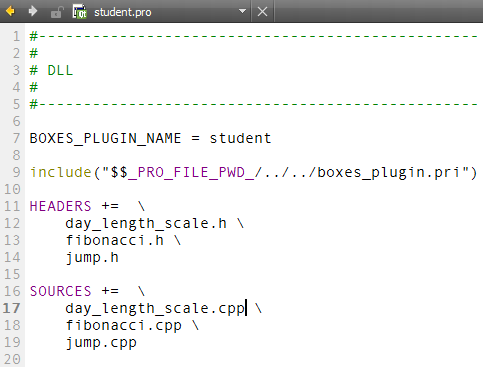
\includegraphics[scale=0.7]{graphics/qt-creator-project-file-2}
\caption{New header and source files added to student project file (\filename{student.pro}).}
\label{fig:qt-creator-project-file-2}
\end{figure}

\begin{figure}
\centering
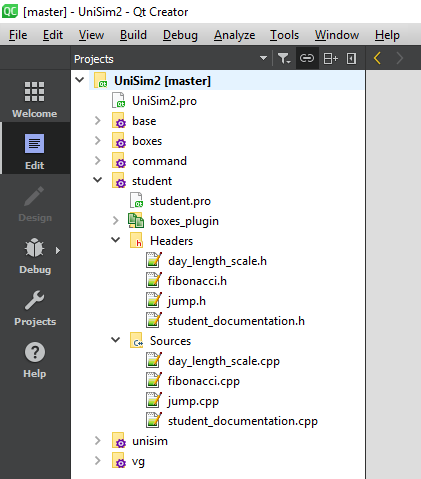
\includegraphics[scale=0.7]{graphics/qt-creator-projects-student-2}
\caption{Projects panel with new header and source files added to the student project.}
\label{fig:qt-creator-projects-student-2}
\end{figure}

After these preliminary steps, we are finally ready to code our \code{DayLengthScale} class. We begin with the header file (\iref{fig:qt-creator-day-length-scale-h}). The arcane embracing of the code (lines 1,2 and 22) reveals the C ancestry of \CPP. The identifier \code{DAY_LENGTH_SCALE} must be unique within the project and is usually set to the class name uppercased. For further explanation you must consult a \CPP\ textbook.

All box classes are based on the \code{Box} base class which is part of the \US\ programming framework. The header file for \code{Box} is included in line 3. Your class will be part of the student plug-in. This is reflected in the \CPP\ code as you put all your code inside the \code{student} namespace (from line 5 to 20). You find the namespace concept in \CPP\ and many other programming languages.

We derive our \code{DayLengthScale} class from the \code{Box} class (line 7) and equip it with three methods (lines 10-12): constructor, \code{reset} and \code{update}. In the private section, we keep data members (or variables); two will serve for input to the box and one will serve as output (lines 13-17).

\begin{figure}
\centering
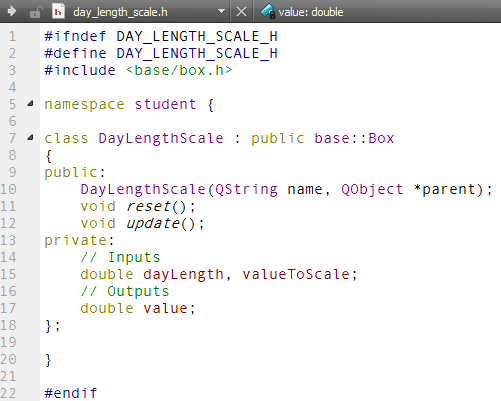
\includegraphics[scale=0.7]{graphics/qt-creator-day-length-scale-h}
\caption{The header file for the \code{DayLengthScale} class found in \filename{\hbox{day_length_scale.h}}.}
\label{fig:qt-creator-day-length-scale-h}
\end{figure}

\begin{figure}
\centering
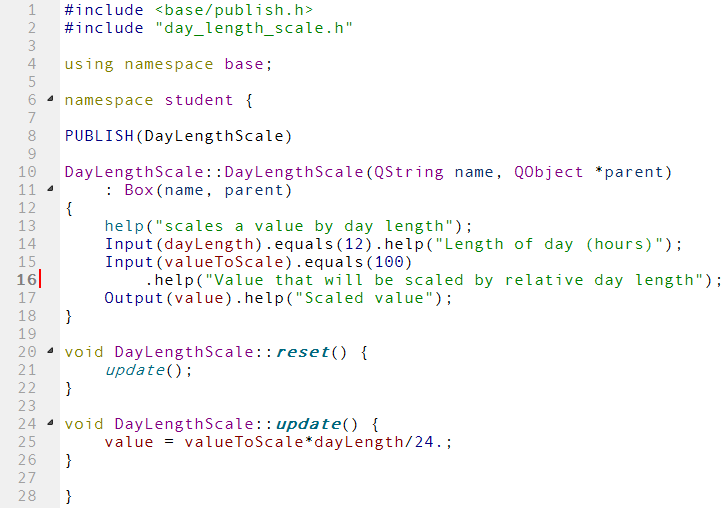
\includegraphics[scale=0.7]{graphics/qt-creator-day-length-scale-cpp}
\caption{The source file for the \code{DayLengthScale} class found in \filename{\hbox{day_length_scale.cpp}}.}
\label{fig:qt-creator-day-length-scale-cpp}
\end{figure}

With all the necessary methods and data members declared in the header file, we are ready to do the actual coding in the source file (\iref{fig:qt-creator-day-length-scale-cpp}).

This source file has the minimum of two \code{include} statements, required for programming a new box class (lines 1-2). One includes the publication mechanism of \US\ which makes it possible to use your class in box scripts. The other is the header file of the class itself which we just wrote.

We open the \code{base} namespace of \US\ to make all code of that namespace directly accessible (line 4). The rest of the code, we put inside our own namespace \code{student} (lines 6-28). We make use of the publication mechanism by \code{PUBLISH}'ing the name of our class (line 8).

The constructor, \code{reset} and \code{update} methods will be called according to the computation model of \US\ (\iref{ch:computations}). Thus \US\ will provide the \code{name} and \code{parent} arguments (line 10) whereever \code{DayLengthObject} is used in a box script. These two arguments are passed on to the \code{Box} base class (line 11).

The two input and one output ports are declared in the constructor using \code{Input} and \code{Output} which technically are not functions but macros (unless you are a programmer, you wouldn't care). The input ports are given default values by the \code{equals} method; if left out the default value is zero. Optionally a brief explanation of a port can be given by the \code{help} method. The \code{help} given in line 13 is a short explanation of the class as a whole. All the help information will be displayed should the user ask for  help at the \US\ prompt (\uscom{help DayLengthScale}). Note how the methods are applied to a port by a dot. The order of method application has no consequence.

When coding the \code{reset} and \code{update} methods the focus, in general, should be on the outputs. In this case, there is only one output, namely \code{value}. In general, you can have other data members than those which hold input and output ports. A simple example is found in the \code{Fibonocci} class also part of the student plug-in. Even though the focus of the whole class is the outputs, if there are other data members then these must also be considered during the reset, update and other computation steps.

The task to carry out in the reset computation step is just to update the box (lines 20-22). The update itself takes the \code{valueToScale} input and scales it by the proportional day length. The result is put in the \code{value} output port (lines 24-26).

\subsection{Use your class in a box script}
To test your newly written box classes you will often start out with quite small and modest box scripts, just to check that it works as expected. In the \filenameexplained{book} folder you will find a series of files from \filename{photo-thermal1.box} to \filename{photo-thermal7.box} with increasing complexity. Here we are taking a closer look at \filename{photo-thermal6.box}:
\lstset{numbers=left}
\begin{boxscript}
// book/photo-thermal6.box
Simulation sim {
  .steps = 365
  Calendar calendar {
    .initialDateTime = 1/1/2009
  }
  Records weather {
    .fileName = "../weather/flakkebjerg 2009.txt"
  }
  Box photoThermalTime {
    +step = ptTimeStep[value]
    DayDegrees dayDegrees {
      .T = weather[Tavg]
      .T0 = 10
    }
    DayLengthScale ptTimeStep {
      .dayLength = calendar[dayLength]
      .valueToScale = dayDegrees[step]
    }
  }
  OutputR {
    PageR {
      .xAxis = calendar[date]
      PlotR {
        .layout = "merged"
        .ports = (weather[Tavg] photoThermalTime[step] 
                  dayDegrees[step])
      }
    }
  }
}\end{boxscript}
\lstset{numbers=none}

The idea here is to let a \code{DayDegrees} box compute the daily day-degree step as usual (lines 12-15), taking the daily average temperature from a weather file managed by a \code{Records} box (lines 7-9). The \code{DayLengthScale} box then takes day length from \code{calendar} and the value to be scaled from \code{dayDegrees} (lines 16-19). 

To give this complexity a nice finish, the \code{dayDegrees} and \code{ptTimeStep} boxes are packaged inside a box with a more describing name \code{photoThermalTime}. We supply this box with an extra port \code{step} which simply refers to the more cryptic \code{ptTimeStep[value]}. Remember that the computation order is children-first (\iref{ch:computations}), so \code{photoThermalTime[step]} will always refer to the most recently calculated \code{ptTimeStep[value]}.

\begin{figure}
\centering
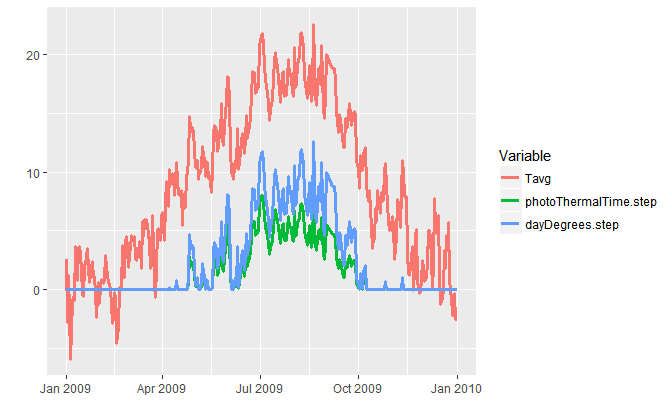
\includegraphics[width=\textwidth]{graphics/photo-thermal-plot1}
\caption{Photo-thermal time calculated by the \filename{photo-thermal06.box} script.}
\label{fig:photo-thermal-plot1}
\end{figure}

The output (\iref{fig:photo-thermal-plot1}) looks as expected. If you wonder what a \code{merged} layout means (line 25), try removing the line and observe the difference in the output.

\section {A simple weather generator}

Sometimes it would be nice to use weather data without all the variability introduced by real weather. Such synthetic data can make it easier during model development because you get a cleaner picture of your model's behaviour without the disturbances of weather variability. The simplest weather generator would just set its outputs to fixed values. Here we will add a tad of sophistication using a sine wave to generate temperature over the year.

As before, we start out copying the \filename{fibonnaci.h} and \filename{fibonacci.cpp} files into \filename{weather.h} and \filename{weather.cpp}. We add these two new files to the \filename{student.pro} project file and end up with a larger project (\iref{fig:qt-creator-projects-student-3}).

\begin{figure}
\centering
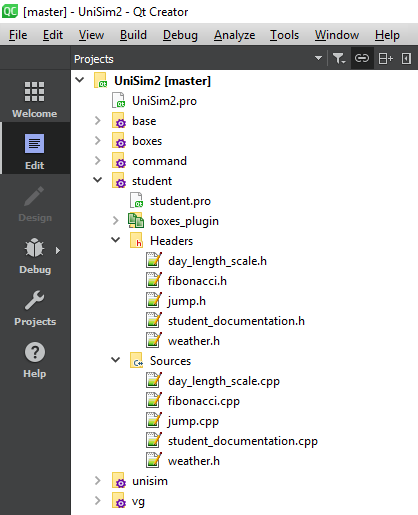
\includegraphics[scale=0.7]{graphics/qt-creator-projects-student-3}
\caption{Projects panel with header and source files for the \code{Weather} class added to the \filename{student} project.}
\label{fig:qt-creator-projects-student-3}
\end{figure}

In the header file (\iref{fig:qt-creator-weather-h}) we declare three methods as for the \code{DayLengthScale} class: constructor, \code{reset} and \code{update} (lines 10-12). For this class we will need four inputs and one output (lines 14-18).

Again, we code all the functionality (or behaviour) of our class in the source file (\iref{fig:qt-creator-weather-cpp}). We give the yearly minimum and maximum temperature some sensible default values (lines 14-15). The coldest day by default we set to 30 (line 16), \ie\ 30 January. The \code{dayOfYear} input we invite the user of the class to set (\ie\ in the box script) by defaulting it implicitly to zero (line 17). If you do not set an explicit default value (with the \code{equals} method) the default is zero. 

At reset there is nothing special to do in addition to updating the box (lines 21-23). The \code{update} method applies  simple trigonometry to obtain a sine wave spanning 365 days with a minimum at \code{dayTmin} (lines 25-29).

After building our project in Qt Creator (it usually requires a few attempts before all typos are weeded out), we write a box script to test our new class. We make it quite simple:
\lstset{numbers=left}
\begin{boxscript}
// book/student-weather.box
Simulation sim {
  .steps = 365
  Calendar calendar {
    .initialDateTime = 1/1/2016
  }
  student::Weather weather {
    .dayOfYear = calendar[dayOfYear]
  }
  OutputR {
    PageR {
      PlotR {
        .ports = weather[T]
      }
    }
  }
}
\end{boxscript}
\lstset{numbers=none}

You should take notice, though, of line 7. Here we qualified the class name by its namespace: \code{student::Weather}. Try to remove the namespace (just keep \code{Weather}) and load the script. You will get an error because another plugin also contains a class named \code{Weather}. This forces us to use the namespace qualification to point out which \code{Weather} we want to use here.

\begin{figure}
\centering
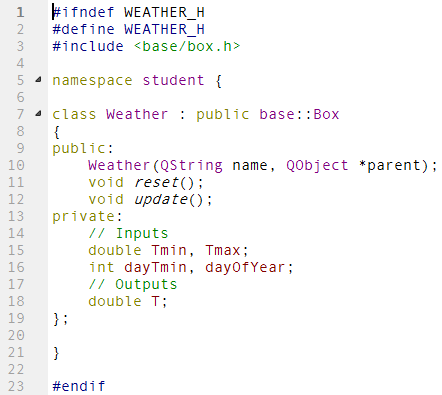
\includegraphics[scale=0.7]{graphics/qt-creator-weather-h}
\caption{The header file for the \code{Weather} class found in \filename{\hbox{weather.h}}.}
\label{fig:qt-creator-weather-h}
\end{figure}

\begin{figure} [bh]
\centering
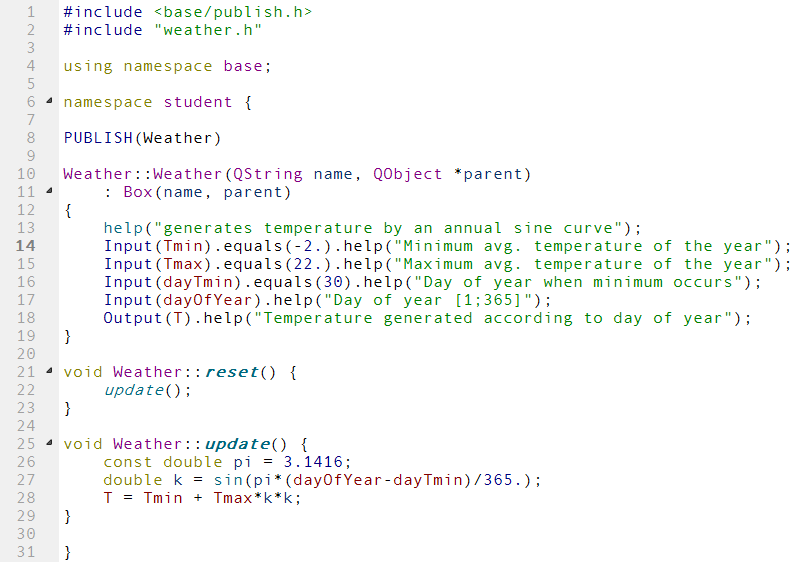
\includegraphics[scale=0.7]{graphics/qt-creator-weather-cpp}
\caption{The source file for the \code{Weather} class found in \filename{\hbox{weather.cpp}}.}
\label{fig:qt-creator-weather-cpp}
\end{figure}

The output of the \filename{weather.box} script is unremarkable so we proceed quickly to combine \code{DayLengthScale} and \code{Weather} in one box script:

\lstset{numbers=left}
\begin{boxscript}
// book/photo-thermal7.box
Simulation sim {
  .steps = 365
  Calendar calendar {
    .initialDateTime = 1/1/2009
  }
  student::Weather weather {
    .dayOfYear = calendar[dayOfYear]
  }
  Box photoThermalTime {
    +step = ptTimeStep[value]
    DayDegrees dayDegrees {
      .T = weather[T]
      .T0 = 10
    }
    DayLengthScale ptTimeStep {
      .dayLength = calendar[dayLength]
      .valueToScale = dayDegrees[step]
    }
  }
  OutputR {
    PageR {
      .xAxis = calendar[date]
      PlotR {
        .layout = "merged"
        .ports = (weather[T] photoThermalTime[step] dayDegrees[step])
      }
    }
  }
}\end{boxscript}
\lstset{numbers=none}

Only little has changed in the box script above, yet the output is remarkably different (\iref{fig:photo-thermal-plot2}. Photo-thermal time is seen to peak a little earlier than day-degree time. That is simply because day length peaks earlier than temperature. Perhaps we had realised that already before carrying out the simulation, or maybe not.

\begin{figure}
\centering
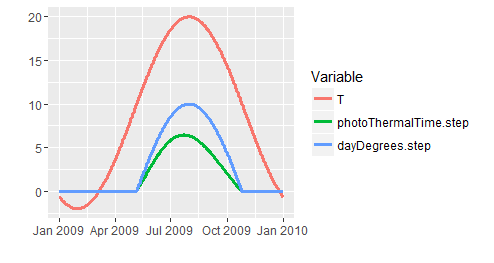
\includegraphics[width=\textwidth]{graphics/photo-thermal-plot2}
\caption{Photo-thermal time calculated by the \filename{photo-thermal07.box} script using a yearly sine-wave for temperature.}
\label{fig:photo-thermal-plot2}
\end{figure}
